\documentclass[10pt, french]{beamer}

% --- Themes and Colors ---
\usetheme{Madrid} % Clean and classic theme
\usecolortheme{whale} % Professional blue palette

% --- Encoding and Language ---
\usepackage[utf8]{inputenc}
\usepackage[T1]{fontenc}
\usepackage{babel}
\usepackage{booktabs}
\usepackage{tikz}
\usetikzlibrary{shapes.geometric, arrows, positioning}

% --- Document Information ---
\title[Titre Court]{Information Retrieval in the Medical Domain: A Comparative
Study on TREC-COVID}
\subtitle{Hands on NLP}
\author[Hands on NLP]{Lounès KEBDI - Lubin LONGUEPEE - Raphael LEONARDI}
\date{\today}

% --- Document Start ---
\begin{document}

% Title page
\begin{frame}
    \titlepage
\end{frame}

% Automatic table of contents


\section{Presentation of the project}

\begin{frame}{Introduction} \begin{columns}[T]

\begin{column}{0.5\textwidth}
\textbf{Context:} \begin{itemize} \item TREC-COVID challenge \item 171,000+ scientific papers \end{itemize}

\vspace{0.5cm}

\textbf{Limitations:} \begin{itemize} \item Exact-match systems (TF-IDF) fail \item Poor retrieval performance \item Semantic gap \end{itemize} \end{column}

\begin{column}{0.5\textwidth}
\centering
\scalebox{0.5}{
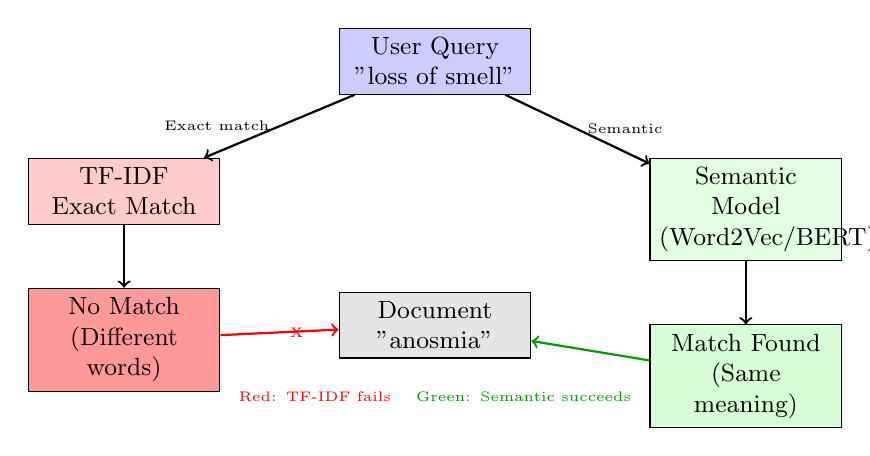
\begin{tikzpicture}[node distance=1cm, auto, font=\small]
    % User query
    \node[rectangle, draw, fill=blue!20, text width=2.2cm, align=center] (query) {User Query\\"loss of smell"};
    
    % TF-IDF path
    \node[rectangle, draw, fill=red!20, text width=2.2cm, align=center, below left=0.8cm and 1.5cm of query] (tfidf) {TF-IDF\\Exact Match};
    \node[rectangle, draw, fill=red!40, text width=2.2cm, align=center, below=0.8cm of tfidf] (tfidf_fail) {No Match\\(Different words)};
    
    % Semantic path
    \node[rectangle, draw, fill=green!10, text width=2.2cm, align=center, below right=0.8cm and 1.5cm of query] (semantic) {Semantic Model\\(Word2Vec/BERT)};
    \node[rectangle, draw, fill=green!15, text width=2.2cm, align=center, below=0.8cm of semantic] (semantic_success) {Match Found\\(Same meaning)};
    
    % Document
    \node[rectangle, draw, fill=gray!20, text width=2.2cm, align=center, below=2.5cm of query] (doc) {Document\\"anosmia"};
    
    % Arrows
    \draw[->, thick] (query) -- node[left, font=\tiny] {Exact match} (tfidf);
    \draw[->, thick] (tfidf) -- (tfidf_fail);
    \draw[->, thick, red] (tfidf_fail) -- node[right, font=\tiny] {\textcolor{red}{X}} (doc);
    
    \draw[->, thick] (query) -- node[right, font=\tiny] {Semantic} (semantic);
    \draw[->, thick] (semantic) -- (semantic_success);
    \draw[->, thick, green!60!black] (semantic_success) -- node[left, font=\tiny] {\textcolor{green!60!black}{$\checkmark$}} (doc);
    
    % Legend
    \node[below=0.3cm of doc, text width=5cm, align=center, font=\tiny] {\textcolor{red}{Red: TF-IDF fails} \quad \textcolor{green!60!black}{Green: Semantic succeeds}};
\end{tikzpicture}
}
\end{column}

\end{columns} \end{frame}


\begin{frame}{Approaches }
    To solve the problem, we have used different approaches, that we will present to you :
    \begin{itemize}
        \item \textbf{Baseline : } TF-IDF (Term Frequency-Inverse Document Fre-
quency)
     \item \textbf{Static Embeddings}: Word2Vec trained on the corpus vs.
Pre-trained BioWord2Vec.
\item \textbf{Neural Models}: Deep Averaging Network (DAN) with
        triplet loss.
    \item \textbf{Transformer Models:} BioBERT (standard) and Sentence-
BERT (optimized for semantic similarity)
    \end{itemize}
\end{frame}

\begin{frame}{Dataset and Methodology}
\begin{block}{TREC-Covid}
    The dataset we used is the TREC-COVID, a dataset created specifically as an information retrieval task 
on Kaggle in 2020. The creators of the dataset, a group of researchers from the NIST published in 2021 an article describing the dataset and the task : \href{https://arxiv.org/abs/2104.09632}{\textbf{Searching for Scientific Evidence in a Pandemic: An Overview of TREC-COVID}}
\end{block}
It contains : 
\begin{itemize}
    \item \textbf{Corpus}: 171,332 scientific articles from the CORD-19 collection, each containing a title and text (abstract or full
content).
\item \textbf{Queries}: 50 distinct topics in natural language, representing real-world information needs.

\item \textbf{Qrels}: Expert relevance judgments used as Ground Truth,
with relevance scores on a -1-2 scale (-1: Document not
evaluate, 0: not relevant, 1: partially relevant, 2: highly
relevant). They are used to evaluate a model, by comparing the relevance predicted by the model to the relevance the experts pointed out.

\end{itemize}
\end{frame}

\begin{frame}{Models}

\begin{block}{TF-IDF}
    
     The first model we use is a TF-IDF, implemented using the scikit-learn TfidfVectorizer with default parameters. \\
   
\end{block}
\begin{block}{Word2Vec Variants.}
\begin{enumerate}
    \item \textbf{W2V-General:} Trained with Gensim’s Word2Vec. Parameters: 200-dimensional embeddings, window size 5, minimum word count 2, trained for 5 epochs.
    \item \textbf{BioWord2Vec}: Pre-trained model trained on 1.5 million biomedical words. Does not use our dataset.
    \item \textbf{BioWord2Vec Fine-tuned:} The pre-trained BioWord2Vec
model further fine-tuned on TREC-COVID for 5 epochs.
    
\end{enumerate}
 For all Word2Vec variants, documents are represented by averaging word embedding, combining title and text.
    
\end{block}
    
\end{frame}

\begin{frame}{Models}
\centering
\scalebox{0.75}{
\begin{tikzpicture}[node distance=1.5cm, auto]
    % Input text (top left)
    \node[rectangle, draw, fill=blue!20, text width=2.2cm, align=center] (input) {Text\\"loss of smell"};
    
    % Tokenization (top center)
    \node[rectangle, draw, fill=yellow!20, text width=2.2cm, align=center, right=1.5cm of input] (token) {Tokenization\\["loss", "smell"]};
    
    % Embeddings (top right)
    \node[rectangle, draw, fill=orange!20, text width=2.2cm, align=center, right=1.5cm of token] (embed) {BioWord2Vec\\Embeddings\\200d each};
    
    % Average (bottom right)
    \node[circle, draw, fill=purple!20, text width=1.8cm, align=center, below=1.2cm of embed] (avg) {Average\\200d};
    
    % MLP (bottom center)
    \node[rectangle, draw, fill=green!20, text width=2.5cm, align=center, left=1.5cm of avg] (mlp) {MLP\\
    Linear(200$\to$300)\\
    ReLU + Dropout\\
    Linear(300$\to$200)};
    
    % Output (bottom left)
    \node[rectangle, draw, fill=red!20, text width=2.2cm, align=center, left=1.5cm of mlp] (output) {Output\\Embedding\\200d};
    
    % Arrows (serpent path)
    \draw[->, thick] (input) -- (token);
    \draw[->, thick] (token) -- (embed);
    \draw[->, thick] (embed) -- (avg);
    \draw[->, thick] (avg) -- (mlp);
    \draw[->, thick] (mlp) -- (output);
\end{tikzpicture}
}

\vspace{0.3cm}
\textbf{Bi-encoder architecture:} Queries and documents share the same encoder.

\textbf{Training data:} Triplets (query, positive document, negative document) encode semantic relationships.
\end{frame}

\begin{frame}{Transformer Models}
\begin{block}{Models}
     \begin{enumerate}
        \item \textbf{BioBERT (Standard):} We used the
        \textit{dmis-lab/biobert-base-cased-v1.1} model from Hugging Face.
        Documents and queries are tokenized with a maximum length of 512
        tokens. We extract the [CLS] token embedding (768 dimensions) as
        the document/query representation. No fine-tuning was performed
        for the retrieval task.

        \item \textbf{Sentence-BERT (S-PubMedBert):} We used \textit{pritamdeka/S-PubMedBert-MS},
        a Siamese BERT network fine-tuned on MS-MARCO (general IR)
        and PubMed (biomedical domain).
     \end{enumerate}
\end{block}

\vspace{0.3cm}
\textbf{Key Difference:} Sentence-BERT embeddings are optimized for
semantic similarity through contrastive learning on pairs of similar/dissimilar texts. BioBERT's [CLS] token is trained for classification tasks, not similarity search.
\end{frame}
\begin{frame}{Evaluation and Performance Comparison}

    \begin{itemize}
        \item \textbf{Evaluation Metric:} NDCG@10 (Normalized Discounted Cumulative Gain at 10)
        \begin{itemize}
            \item Prioritizes highly relevant documents at the top of the ranking list.
            \item Accounts for both relevance and ranking position, making it ideal for IR evaluation.
            \item Reported: Mean NDCG@10 across all 50 queries, with standard deviation, minimum, and maximum scores.
        \end{itemize}
    \end{itemize}

    \vspace{0.5cm}
    
    \centering
    \renewcommand{\arraystretch}{1.2}
    \begin{tabular}{l | c c c c}
  \textbf{Model} & \textbf{Mean} & \textbf{Std} & \textbf{Min} & \textbf{Max} \\
    \hline
    TF-IDF (Baseline)         & 0.5868 & 0.3350 & 0.0000 & 1.0000 \\
    Word2Vec (Corpus)         & 0.6099 & 0.3301 & 0.0000 & 1.0000 \\
    BioWord2Vec (Pre-trained) & 0.7366 & 0.3029 & 0.0000 & 1.0000 \\
    BioWord2Vec (Fine-tuned)  & 0.6259 & 0.3263 & 0.0000 & 1.0000 \\
    DAN                       & 0.6630 & 0.2696 & 0.0000 & 1.0000 \\
    BioBERT (Standard)        & 0.2886 & 0.3454 & 0.0000 & 1.0000 \\
    \hline
    \textbf{Sentence-BERT}    & \textbf{0.8171} & \textbf{0.2305} & \textbf{0.0000} & \textbf{0.9986} \\
\end{tabular}

\end{frame}


\begin{frame}{Conclusion}
    \begin{block}{Best Model}
        This study evaluated multiple IR strategies for the TREC-COVID
challenge, ranging from classical lexical methods to state-of-the-art
neural architectures. We demonstrated that Sentence-BERT is
the most effective approach (NDCG@10: 0.8171), leveraging both
domain-specific pretraining and an architecture optimized for semantic similarity.
    \end{block}
\begin{block}{Key Findings}
\begin{enumerate} 
\item \textbf{Domain-specific pre-training is crucial:} BioWord2Vec (+25.5\%) and Sentence-BERT (+39.2\%) significantly outperform generic models.
\item \textbf{Task-specific optimization matters:} Sentence-BERT's similarity-focused training outperforms BioBERT's classification focused embeddings by 183\%.
\item \textbf{Model complexity requires data:} Trainable models (DAN, fine-tuned W2V) underperform simpler approaches when training data is limited (50 queries). \item \textbf{Simple can be effective:} BioWord2Vec averaging (0.7366) outperforms complex neural architectures (DAN: 0.6630) in low-data scenarios. \end{enumerate}
    
\end{block}

    
\end{frame}



\begin{frame}{Thanks you for your attention !}
    \centering
    \Huge Questions ?
\end{frame}

\end{document}